
\subsection{old}

 In this section, we apply ILRT to the normal mixture model.
 is the first example of unbounded likelihood given in~\cite{Cam1990Maximum}.


Suppose $X_1,\ldots,X_n$ are i.i.d.\ distributed as a mixture of normal distributions
\begin{equation}
    p(X|\theta)=\frac{1-\alpha}{\sqrt{2\pi}}\exp\left\{-\frac{1}{2}{(X-\mu)}^2\right\}+
    \frac{\alpha}{\sigma\sqrt{2\pi}}\exp\left\{-\frac{1}{2}\frac{{(X-\mu)}^2}{\sigma^2}\right\},
\end{equation}
 where $\alpha$ is a known constant. Suppose the parameter space is
\begin{equation}
    \Theta=\{\theta={(\mu,\sigma^2)}^T:\mu\in(\-\infty,\infty),\sigma^2\in (0,M)\},
\end{equation}
where $M$ is a sufficiently large parameter.
\cite{Cam1990Maximum} pointed out that the likelihood of the model is unbounded. In fact, let $\mu=X_1$ and let $\sigma^2\to 0$, then the likelihood tends to infinity.

Under the model, we consider testing the hypotheses $H_0:\mu=0,\sigma=2$ vs $H_1:\theta\in
\Theta$. Although LRT fails in this model, ILRT can still be used. To use ILRT, we need a weight function.
First let the weight function be the posterior density of parameters. To make the posterior density bounded from infinity, we consider the so-called zero-avoiding prior. See~\cite{bayesianDataAnalysis} section 13.2.
When $\mu=X_1$, as $\sigma^2\to 0$, the likelihood tends to infinity at the rate of ${1}/{\sigma}$. The rate can be hedged by the density of $\chi^2_3$. Hence we adopt the following prior distribution

\begin{equation}
    \phi(\mu)\times d\chi^2_3(\sigma^2),
\end{equation}
where $d\chi^2_3(\sigma^2)$ represents the density of $\chi^2$ distribution with freedom $3$ taking value at $\sigma^2$. Because the $\sigma^2$ is limited in $(0,M)$, we also truncate prior of $\sigma^2$ at $M$.

 We take sample size $n=50,100,200$ and $\alpha=0.1,0.5,0.9$. In every combination, we repeat $1000$ samples and obtain $1000$ ILRT statistics.
 We expect the empirical distribution of $2\log \Lambda_{a,b}(\BX^{(n)})$ is similar to that of $-2\log 2+\chi^2_2$.
 We plot the QQ-plot of empirical distribution relative to  $-2\log 2+\chi^2_2$ distribution, it can be seen that ILRT can be well approximated by $\chi^2(2)$.

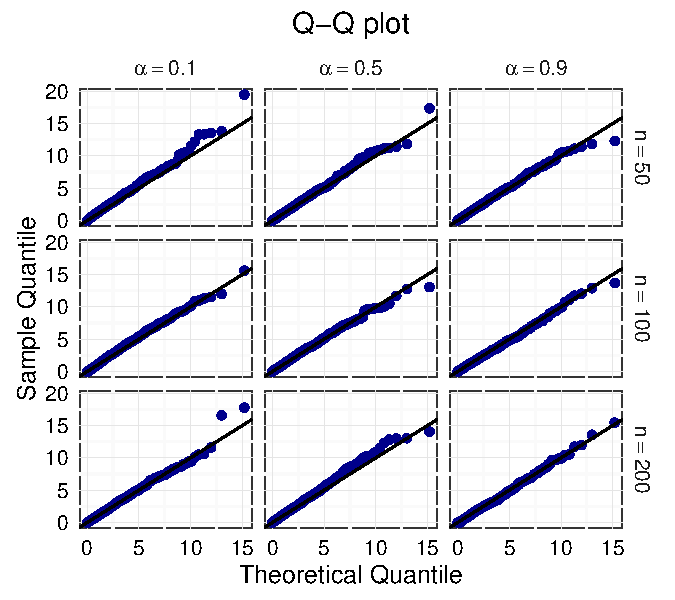
\includegraphics{myQQPlot.pdf}


Next we consider another weight function $\pi (\theta; X)= N(\hat{\theta},\frac{1}{n}\hat{I}^{-1}_{\hat{\theta}})$. Lt $\hat{\theta}$ be the highest probability density estimator. And 
$$\hat{I}_\theta^{-1}=\sum_{i=1}^n
\begin{bmatrix}
-\frac{\partial^2 \log p_\theta(x_i)}{\partial \mu^2}&
    -\frac{\partial^2 \log p_\theta(x_i)}{\partial \mu\partial (\sigma^2)}
\\
    -\frac{\partial^2 \log p_\theta(x_i)}{\partial \mu\partial (\sigma^2)}
    &
    -\frac{\partial^2 \log p_\theta(x_i)}{\partial {(\sigma^2)}^2}
\end{bmatrix}$$
where

\begin{equation}
    \begin{aligned}
\frac{\partial^2 \log p_\theta(x)}{\partial
        \mu^2}=&
        \frac{(1-\alpha)({(x-\mu)}^2-1)dN(\mu,1)(x)+\alpha ({(x-\mu)}^2/\sigma^4 -\sigma^{-2})dN(\mu,\sigma^2)(x)}{p_\theta (x)}-\\
        &
        {\Big(\frac{(1-\alpha)(x-\mu)dN(\mu,1)(x)+\alpha(x-\mu)/\sigma^2 dN(\mu,\sigma^2)(x)}{p_\theta(x)}\Big)}^2,
    \end{aligned}
\end{equation}

\begin{equation}
    \begin{aligned}
        &\frac{\partial^2 \log p_\theta(x)}{\partial
        \mu\partial(\sigma^2)}=
        \frac{(\frac{3\alpha(\mu-x)}{2\sigma^4}-\frac{\alpha {(\mu-x)}^3}{2\sigma^6})dN(\mu,\sigma^2)(x)}{p_\theta (x)}-\\
        &
        \frac{\alpha (\frac{{(\mu-x)}^2}{2\sigma^4}-\frac{1}{2\sigma^2})dN(\mu,\sigma^2)(x)\big((1-\alpha)(x-\mu)dN(\mu,1)(x)+\alpha(x-\mu)/\sigma^2 d(\mu,\sigma^2)(x)\big)}{p_{\theta}{(x)}^2},
    \end{aligned}
\end{equation}


\begin{equation}
    \begin{aligned}
\frac{\partial^2 \log p_\theta(x)}{\partial
        {(\sigma^2)}^2}=&
        \frac{\alpha \big(\frac{3}{4\sigma^4}-\frac{3{(x-\mu)}^2}{2\sigma^6} +\frac{{(x-\mu)}^4}{4\sigma^8}\big)dN(\mu,\sigma^2)(x)}{p_\theta (x)}-\\
        &
        {\Big(\frac{\alpha\big(\frac{{(x-\mu)}^2}{2\sigma^4}-\frac{1}{2\sigma^2} \big)dN(\mu,\sigma^2)(x)}{p_\theta(x)}\Big)}^2.
    \end{aligned}
\end{equation}

We do the same simulation as above and the QQ-plot is given.
It  can be seen that the distribution of ILRT statistic is still close to the theoretical distribution in this case.
For mixture model, sampling from posterior distribution is troublesome.
The computing burden will be reduce by normal approximation.
This is an advantage of normal weight ILRT.\@ From this example, we can see that ILRT is more flexible than posterior Bayes factor.


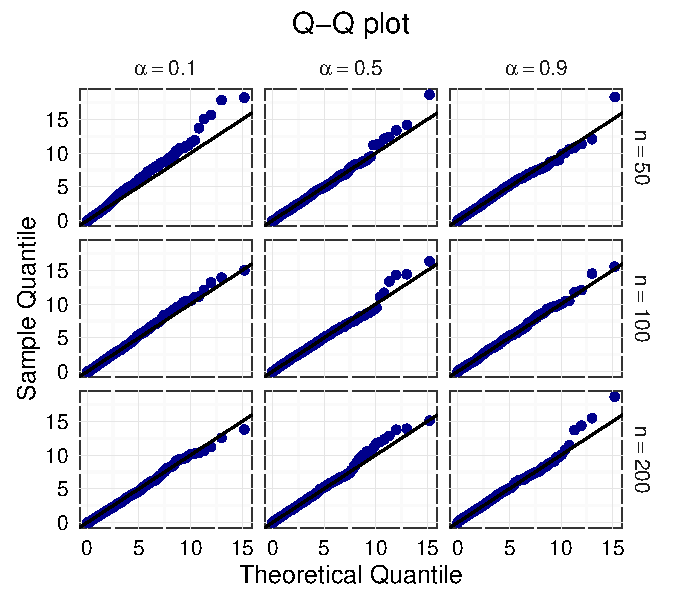
\includegraphics{myQQPlotNormal.pdf}


